\documentclass[12pt,openany]{book}
\usepackage{lmodern}
\usepackage{amssymb,amsmath}
\usepackage{ifxetex,ifluatex}
\usepackage{fixltx2e} % provides \textsubscript
\usepackage{calc} % For simpler calculation - used for spacing the index letter headings correctly


%----------------------------------------------------------------------------------------
%	VARIOUS REQUIRED PACKAGES AND CONFIGURATIONS
%----------------------------------------------------------------------------------------

\usepackage{graphicx} % Required for including pictures
\graphicspath{{Pictures/}} % Specifies the directory where pictures are stored

\usepackage{tikz} % Required for drawing custom shapes

\usepackage[english]{babel} % English language/hyphenation

\usepackage{enumitem} % Customize lists
\setlist{nolistsep} % Reduce spacing between bullet points and numbered lists

\usepackage{booktabs} % Required for nicer horizontal rules in tables

\usepackage{xcolor} % Required for specifying colors by name
%\definecolor{ocre}{RGB}{243,102,25} % Define the orange color used for highlighting throughout the book
\definecolor{ocre}{RGB}{85, 165, 250} % Define the blue color used for highlighting throughout the book

\usepackage{avant} % Use the Avantgarde font for headings
%\usepackage{times} % Use the Times font for headings
\usepackage{mathptmx} % Use the Adobe Times Roman as the default text font together with math symbols from other fonts

\usepackage{microtype} % Slightly tweak font spacing for aesthetics
\usepackage[utf8]{inputenc} % Required for including letters with accents
\usepackage[T1]{fontenc} % Use 8-bit encoding that has 256 glyphs
\usepackage{textcomp}

%----------------------------------------------------------------------------------------
%	MAIN TABLE OF CONTENTS
%----------------------------------------------------------------------------------------

\usepackage{titletoc} % Required for manipulating the table of contents

\contentsmargin{0cm} % Removes the default margin

% Part text styling (this is mostly taken care of in the PART HEADINGS section of this file)
\titlecontents{part}
	[0cm] % Left indentation
	{\addvspace{20pt}\bfseries} % Spacing and font options for parts
	{}
	{}
	{}

% Chapter text styling
\titlecontents{chapter}
	[1.25cm] % Left indentation
	{\addvspace{12pt}\large\sffamily\bfseries} % Spacing and font options for chapters
	{\color{ocre!60}\contentslabel[\Large\thecontentslabel]{1.25cm}\color{ocre}} % Formatting of numbered sections of this type
	{\color{ocre}} % Formatting of numberless sections of this type
	{\color{ocre!60}\normalsize\;\titlerule*[.5pc]{.}\;\thecontentspage} % Formatting of the filler to the right of the heading and the page number

% Section text styling
\titlecontents{section}
	[1.25cm] % Left indentation
	{\addvspace{3pt}\sffamily\bfseries} % Spacing and font options for sections
	{\contentslabel[\thecontentslabel]{1.25cm}} % Formatting of numbered sections of this type
	{} % Formatting of numberless sections of this type
	{\hfill\color{black}\thecontentspage} % Formatting of the filler to the right of the heading and the page number

% Subsection text styling
\titlecontents{subsection}
	[1.25cm] % Left indentation
	{\addvspace{1pt}\sffamily\small} % Spacing and font options for subsections
	{\contentslabel[\thecontentslabel]{1.25cm}} % Formatting of numbered sections of this type
	{} % Formatting of numberless sections of this type
	{\ \titlerule*[.5pc]{.}\;\thecontentspage} % Formatting of the filler to the right of the heading and the page number

% Figure text styling
\titlecontents{figure}
	[1.25cm] % Left indentation
	{\addvspace{1pt}\sffamily\small} % Spacing and font options for figures
	{\thecontentslabel\hspace*{1em}} % Formatting of numbered sections of this type
	{} % Formatting of numberless sections of this type
	{\ \titlerule*[.5pc]{.}\;\thecontentspage} % Formatting of the filler to the right of the heading and the page number

% Table text styling
\titlecontents{table}
	[1.25cm] % Left indentation
	{\addvspace{1pt}\sffamily\small} % Spacing and font options for tables
	{\thecontentslabel\hspace*{1em}} % Formatting of numbered sections of this type
	{} % Formatting of numberless sections of this type
	{\ \titlerule*[.5pc]{.}\;\thecontentspage} % Formatting of the filler to the right of the heading and the page number
	
%----------------------------------------------------------------------------------------
%	MINI TABLE OF CONTENTS IN PART HEADS
%----------------------------------------------------------------------------------------

% Chapter text styling
\titlecontents{lchapter}
	[0em] % Left indentation
	{\addvspace{15pt}\large\sffamily\bfseries} % Spacing and font options for chapters
	{\color{ocre}\contentslabel[\Large\thecontentslabel]{1.25cm}\color{ocre}} % Chapter number
	{}  
	{\color{ocre}\normalsize\sffamily\bfseries\;\titlerule*[.5pc]{.}\;\thecontentspage} % Page number

% Section text styling
\titlecontents{lsection}
	[0em] % Left indentation
	{\sffamily\small} % Spacing and font options for sections
	{\contentslabel[\thecontentslabel]{1.25cm}} % Section number
	{}
	{}

% Subsection text styling (note these aren't shown by default, display them by searchings this file for tocdepth and reading the commented text)
\titlecontents{lsubsection}
	[.5em] % Left indentation
	{\sffamily\footnotesize} % Spacing and font options for subsections
	{\contentslabel[\thecontentslabel]{1.25cm}}
	{}
	{}


% \ifnum 0\ifxetex 1\fi\ifluatex 1\fi=0 % if pdftex
%   \usepackage[T1]{fontenc}
%   \usepackage[utf8]{inputenc}
% % \else % if luatex or xelatex
%   \ifxetex
%     \usepackage{mathspec}
%   \else
%     \usepackage{fontspec}
%   \fi
%   \defaultfontfeatures{Ligatures=TeX,Scale=MatchLowercase}
% % % % % % % \fi
% % use upquote if available, for straight quotes in verbatim environments
% \IfFileExists{upquote.sty}{\usepackage{upquote}}{}
% % use microtype if available
% \IfFileExists{microtype.sty}{%
% \usepackage{microtype}
% \UseMicrotypeSet[protrusion]{basicmath} % disable protrusion for tt fonts
% }{}
\usepackage[margin=1in]{geometry}


%----------------------------------------------------------------------------------------
%	HEADERS AND FOOTERS
%----------------------------------------------------------------------------------------

\usepackage{fancyhdr} % Required for header and footer configuration

\pagestyle{fancy} % Enable the custom headers and footers

\renewcommand{\chaptermark}[1]{\markboth{\sffamily\normalsize\bfseries\chaptername\ \thechapter.\ #1}{}} % Styling for the current chapter in the header
\renewcommand{\sectionmark}[1]{\markright{\sffamily\normalsize\thesection\hspace{5pt}#1}{}} % Styling for the current section in the header

\fancyhf{} % Clear default headers and footers
\fancyhead[LE,RO]{\sffamily\normalsize\thepage} % Styling for the page number in the header
\fancyhead[LO]{\rightmark} % Print the nearest section name on the left side of odd pages
\fancyhead[RE]{\leftmark} % Print the current chapter name on the right side of even pages
%\fancyfoot[C]{\thepage} % Uncomment to include a footer

\renewcommand{\headrulewidth}{0.5pt} % Thickness of the rule under the header

\fancypagestyle{plain}{% Style for when a plain pagestyle is specified
	\fancyhead{}\renewcommand{\headrulewidth}{0pt}%
}

% Removes the header from odd empty pages at the end of chapters
\makeatletter
\renewcommand{\cleardoublepage}{
\clearpage\ifodd\c@page\else
\hbox{}
\vspace*{\fill}
\thispagestyle{empty}
\newpage
\fi}

%----------------------------------------------------------------------------------------
%	THEOREM STYLES
%----------------------------------------------------------------------------------------

\usepackage{amsmath,amsfonts,amssymb,amsthm} % For math equations, theorems, symbols, etc

\newcommand{\intoo}[2]{\mathopen{]}#1\,;#2\mathclose{[}}
\newcommand{\ud}{\mathop{\mathrm{{}d}}\mathopen{}}
\newcommand{\intff}[2]{\mathopen{[}#1\,;#2\mathclose{]}}
\newtheorem{notation}{Notation}[chapter]

% Boxed/framed environments
\newtheoremstyle{ocrenumbox}% Theorem style name
{0pt}% Space above
{0pt}% Space below
{\normalfont}% Body font
{}% Indent amount
{\small\bf\sffamily\color{ocre}}% Theorem head font
{\;}% Punctuation after theorem head
{0.25em}% Space after theorem head
{\small\sffamily\color{ocre}\thmname{#1}\nobreakspace\thmnumber{\@ifnotempty{#1}{}\@upn{#2}}% Theorem text (e.g. Theorem 2.1)
\thmnote{\nobreakspace\the\thm@notefont\sffamily\bfseries\color{black}---\nobreakspace#3.}} % Optional theorem note

\newtheoremstyle{blacknumex}% Theorem style name
{5pt}% Space above
{5pt}% Space below
{\normalfont}% Body font
{} % Indent amount
{\small\bf\sffamily}% Theorem head font
{\;}% Punctuation after theorem head
{0.25em}% Space after theorem head
{\small\sffamily{\tiny\ensuremath{\blacksquare}}\nobreakspace\thmname{#1}\nobreakspace\thmnumber{\@ifnotempty{#1}{}\@upn{#2}}% Theorem text (e.g. Theorem 2.1)
\thmnote{\nobreakspace\the\thm@notefont\sffamily\bfseries---\nobreakspace#3.}}% Optional theorem note

\newtheoremstyle{blacknumbox} % Theorem style name
{0pt}% Space above
{0pt}% Space below
{\normalfont}% Body font
{}% Indent amount
{\small\bf\sffamily}% Theorem head font
{\;}% Punctuation after theorem head
{0.25em}% Space after theorem head
{\small\sffamily\thmname{#1}\nobreakspace\thmnumber{\@ifnotempty{#1}{}\@upn{#2}}% Theorem text (e.g. Theorem 2.1)
\thmnote{\nobreakspace\the\thm@notefont\sffamily\bfseries---\nobreakspace#3.}}% Optional theorem note

% Non-boxed/non-framed environments
\newtheoremstyle{ocrenum}% Theorem style name
{5pt}% Space above
{5pt}% Space below
{\normalfont}% Body font
{}% Indent amount
{\small\bf\sffamily\color{ocre}}% Theorem head font
{\;}% Punctuation after theorem head
{0.25em}% Space after theorem head
{\small\sffamily\color{ocre}\thmname{#1}\nobreakspace\thmnumber{\@ifnotempty{#1}{}\@upn{#2}}% Theorem text (e.g. Theorem 2.1)
\thmnote{\nobreakspace\the\thm@notefont\sffamily\bfseries\color{black}---\nobreakspace#3.}} % Optional theorem note
\makeatother

% Non-boxed/non-framed environments
\newtheoremstyle{ocrenumb}% Theorem style name
{5pt}% Space above
{5pt}% Space below
{\normalfont}% Body font
{}% Indent amount
{\small\bf\sffamily\color{ocre}}% Theorem head font
{\;}% Punctuation after theorem head
{0pt}% Space after theorem head
% {\small\sffamily\color{ocre}\thmname{#1}\nobreakspace\thmnumber{\@ifnotempty{#1}{}\@upn{#2}}% Theorem text (e.g. Theorem 2.1)
% \thmnote{\nobreakspace\the\thm@notefont\sffamily\bfseries\color{black}---\nobreakspace#3.}} % Optional theorem note
\makeatother


% Defines the theorem text style for each type of theorem to one of the three styles above
\newcounter{dummy} 
\numberwithin{dummy}{section}
\theoremstyle{ocrenumbox}
\newtheorem{theoremeT}[dummy]{Theorem}
\newtheorem{problem}{Problem}[chapter]
\newtheorem{exerciseT}{Exercise}[chapter]
\theoremstyle{ocrenumb}
\newtheorem*{blankexerciseT}{}
\theoremstyle{blacknumex}
\newtheorem{exampleT}{Example}[chapter]
\theoremstyle{blacknumbox}
\newtheorem{vocabulary}{Vocabulary}[chapter]
\newtheorem{definitionT}{Definition}[section]
\newtheorem{corollaryT}[dummy]{Corollary}
\theoremstyle{ocrenum}
\newtheorem{proposition}[dummy]{Proposition}

%----------------------------------------------------------------------------------------
%	DEFINITION OF COLORED BOXES
%----------------------------------------------------------------------------------------

\RequirePackage[framemethod=default]{mdframed} % Required for creating the theorem, definition, exercise and corollary boxes

% Theorem box
\newmdenv[skipabove=7pt,
skipbelow=7pt,
backgroundcolor=black!5,
linecolor=ocre,
innerleftmargin=5pt,
innerrightmargin=5pt,
innertopmargin=5pt,
leftmargin=0cm,
rightmargin=0cm,
innerbottommargin=5pt]{tBox}

% Exercise box	  
\newmdenv[skipabove=7pt,
skipbelow=7pt,
rightline=false,
leftline=true,
topline=false,
bottomline=false,
backgroundcolor=ocre!10,
linecolor=ocre,
innerleftmargin=5pt,
innerrightmargin=5pt,
innertopmargin=5pt,
innerbottommargin=5pt,
leftmargin=0cm,
rightmargin=0cm,
linewidth=4pt]{eBox}	

% Definition box
\newmdenv[skipabove=7pt,
skipbelow=7pt,
rightline=false,
leftline=true,
topline=false,
bottomline=false,
linecolor=ocre,
innerleftmargin=5pt,
innerrightmargin=5pt,
innertopmargin=0pt,
leftmargin=0cm,
rightmargin=0cm,
linewidth=4pt,
innerbottommargin=0pt]{dBox}	

% Corollary box
\newmdenv[skipabove=7pt,
skipbelow=7pt,
rightline=false,
leftline=true,
topline=false,
bottomline=false,
linecolor=gray,
backgroundcolor=black!5,
innerleftmargin=5pt,
innerrightmargin=5pt,
innertopmargin=5pt,
leftmargin=0cm,
rightmargin=0cm,
linewidth=4pt,
innerbottommargin=5pt]{cBox}

% Creates an environment for each type of theorem and assigns it a theorem text style from the "Theorem Styles" section above and a colored box from above
% \newenvironment{theorem}{\begin{tBox}\begin{theoremeT}}{\end{theoremeT}\end{tBox}}
\newenvironment{exercise}{\begin{eBox}\begin{exerciseT}}{\hfill{\color{ocre}\tiny\ensuremath{\blacksquare}}\end{exerciseT}\end{eBox}}				  
\newenvironment{blankexercise}{\begin{eBox}\begin{blankexerciseT}}{\hfill{\color{ocre}\tiny\ensuremath{\blacksquare}}\end{blankexerciseT}\end{eBox}}				  
\newenvironment{definition}{\begin{dBox}\begin{definitionT}}{\end{definitionT}\end{dBox}}	
\newenvironment{example}{\begin{exampleT}}{\hfill{\tiny\ensuremath{\blacksquare}}\end{exampleT}}	
\newenvironment{corollary}{\begin{cBox}\begin{corollaryT}}{\end{corollaryT}\end{cBox}}	

%----------------------------------------------------------------------------------------
%	REMARK ENVIRONMENT
%----------------------------------------------------------------------------------------


\newenvironment{remark}{\begin{eBox}\begin{blankexerciseT}}{\hfill{\color{ocre}\tiny\ensuremath{\blacksquare}}\end{blankexerciseT}\end{eBox}}

% \newenvironment{remark}{\par\vspace{7pt}\small % Vertical white space above the remark and smaller font size
% \begin{list}{}{
% \leftmargin=0pt % Indentation on the left
% \rightmargin=0pt}\item\ignorespaces % Indentation on the right
% \makebox[-2.5pt]{\begin{tikzpicture}[overlay]
% \node[draw=ocre!60,line width=1pt,circle,fill=ocre!25,font=\sffamily\bfseries,inner sep=2pt,outer sep=0pt] at (-15pt,0pt){\textcolor{ocre}{R}};\end{tikzpicture}} % Orange R in a circle
% \advance\baselineskip -1pt}{\end{list}\vskip5pt} % Tighter line spacing and white space after remark


%----------------------------------------------------------------------------------------
%	SECTION NUMBERING IN THE MARGIN
%----------------------------------------------------------------------------------------

\makeatletter
\renewcommand{\@seccntformat}[1]{\llap{\textcolor{ocre}{\csname the#1\endcsname}\hspace{1em}}}                    
\renewcommand{\section}{\@startsection{section}{1}{\z@}
{-4ex \@plus -1ex \@minus -.4ex}
{1ex \@plus.2ex }
{\normalfont\large\sffamily\bfseries}}
\renewcommand{\subsection}{\@startsection {subsection}{2}{\z@}
{-3ex \@plus -0.1ex \@minus -.4ex}
{0.5ex \@plus.2ex }
{\normalfont\sffamily\bfseries}}
\renewcommand{\subsubsection}{\@startsection {subsubsection}{3}{\z@}
{-2ex \@plus -0.1ex \@minus -.2ex}
{.2ex \@plus.2ex }
{\normalfont\small\sffamily\bfseries}}                        
\renewcommand\paragraph{\@startsection{paragraph}{4}{\z@}
{-2ex \@plus-.2ex \@minus .2ex}
{.1ex}
{\normalfont\small\sffamily\bfseries}}
\makeatother


%----------------------------------------------------------------------------------------
%	PART HEADINGS
%----------------------------------------------------------------------------------------

\makeatletter
% Numbered part in the table of contents
\newcommand{\@mypartnumtocformat}[2]{%
	\setlength\fboxsep{0pt}%
	\noindent\colorbox{ocre!20}{\strut\parbox[c][.7cm]{\ecart}{\color{ocre!70}\Large\sffamily\bfseries\centering#1}}\hskip\esp\colorbox{ocre!40}{\strut\parbox[c][.7cm]{\linewidth-\ecart-\esp}{\Large\sffamily\centering#2}}%
}

% Unnumbered part in the table of contents
\newcommand{\@myparttocformat}[1]{%
	\setlength\fboxsep{0pt}%
	\noindent\colorbox{ocre!40}{\strut\parbox[c][.7cm]{\linewidth}{\Large\sffamily\centering#1}}%
}

\newlength\esp
\setlength\esp{4pt}
\newlength\ecart
\setlength\ecart{1.2cm-\esp}
\newcommand{\thepartimage}{}%
\newcommand{\partimage}[1]{\renewcommand{\thepartimage}{#1}}%
\def\@part[#1]#2{%
\ifnum \c@secnumdepth >-2\relax%
\refstepcounter{part}%
\addcontentsline{toc}{part}{\texorpdfstring{\protect\@mypartnumtocformat{\thepart}{#1}}{\partname~\thepart\ ---\ #1}}
\else%
\addcontentsline{toc}{part}{\texorpdfstring{\protect\@myparttocformat{#1}}{#1}}%
\fi%
\startcontents%
\markboth{}{}%
{\thispagestyle{empty}%
\begin{tikzpicture}[remember picture,overlay]%
\node at (current page.north west){\begin{tikzpicture}[remember picture,overlay]%	
\fill[ocre!20](0cm,0cm) rectangle (\paperwidth,-\paperheight);
\node[anchor=north] at (4cm,-3.25cm){\color{ocre!40}\fontsize{220}{100}\sffamily\bfseries\thepart}; 
\node[anchor=south east] at (\paperwidth-1cm,-\paperheight+1cm){\parbox[t][][t]{8.5cm}{
\printcontents{l}{0}{\setcounter{tocdepth}{1}}% The depth to which the Part mini table of contents displays headings; 0 for chapters only, 1 for chapters and sections and 2 for chapters, sections and subsections
}};
\node[anchor=north east] at (\paperwidth-1.5cm,-3.25cm){\parbox[t][][t]{15cm}{\strut\raggedleft\color{black}\fontsize{30}{30}\sffamily\bfseries#2}};
\end{tikzpicture}};
\end{tikzpicture}}%
\@endpart}
\def\@spart#1{%
\startcontents%
\phantomsection
{\thispagestyle{empty}%
\begin{tikzpicture}[remember picture,overlay]%
\node at (current page.north west){\begin{tikzpicture}[remember picture,overlay]%	
\fill[ocre!20](0cm,0cm) rectangle (\paperwidth,-\paperheight);
\node[anchor=north east] at (\paperwidth-1.5cm,-3.25cm){\parbox[t][][t]{15cm}{\strut\raggedleft\color{white}\fontsize{30}{30}\sffamily\bfseries#1}};
\end{tikzpicture}};
\end{tikzpicture}}
\addcontentsline{toc}{part}{\texorpdfstring{%
\setlength\fboxsep{0pt}%
\noindent\protect\colorbox{ocre!40}{\strut\protect\parbox[c][.7cm]{\linewidth}{\Large\sffamily\protect\centering #1\quad\mbox{}}}}{#1}}%
\@endpart}
\def\@endpart{\vfil\newpage
\if@twoside
\if@openright
\null
\thispagestyle{empty}%
\newpage
\fi
\fi
\if@tempswa
\twocolumn
\fi}
\makeatother

%----------------------------------------------------------------------------------------
%	CHAPTER HEADINGS
%----------------------------------------------------------------------------------------

\makeatletter
% A switch to conditionally include a picture, implemented by Christian Hupfer
\newif\ifusechapterimage
\usechapterimagetrue
\newcommand{\thechapterimage}{}%
\newcommand{\chapterimage}[1]{\ifusechapterimage\renewcommand{\thechapterimage}{#1}\fi}%
\newcommand{\autodot}{.}
\def\@makechapterhead#1{%
{\parindent \z@ \raggedright \normalfont
\ifnum \c@secnumdepth >\m@ne
\if@mainmatter
\begin{tikzpicture}[remember picture,overlay]
\node at (current page.north west)
{\begin{tikzpicture}[remember picture,overlay]
\node[anchor=north west,inner sep=0pt] at (0,0) {\ifusechapterimage\includegraphics[width=\paperwidth]{\thechapterimage}\fi};
\draw[anchor=west] (\Gm@lmargin,-9cm) node [line width=2pt,rounded corners=15pt,draw=ocre,fill=white,fill opacity=0.5,inner sep=15pt]{\strut\makebox[22cm]{}};
\draw[anchor=west] (\Gm@lmargin+.3cm,-9cm) node {\huge\sffamily\bfseries\color{black}\thechapter\autodot~#1\strut};
\end{tikzpicture}};
\end{tikzpicture}
\else
\begin{tikzpicture}[remember picture,overlay]
\node at (current page.north west)
{\begin{tikzpicture}[remember picture,overlay]
\node[anchor=north west,inner sep=0pt] at (0,0) {\ifusechapterimage\includegraphics[width=\paperwidth]{\thechapterimage}\fi};
\draw[anchor=west] (\Gm@lmargin,-9cm) node [line width=2pt,rounded corners=15pt,draw=ocre,fill=white,fill opacity=0.5,inner sep=15pt]{\strut\makebox[22cm]{}};
\draw[anchor=west] (\Gm@lmargin+.3cm,-9cm) node {\huge\sffamily\bfseries\color{black}#1\strut};
\end{tikzpicture}};
\end{tikzpicture}
\fi\fi\par\vspace*{270\p@}}}

%-------------------------------------------

\def\@makeschapterhead#1{%
\begin{tikzpicture}[remember picture,overlay]
\node at (current page.north west)
{\begin{tikzpicture}[remember picture,overlay]
\node[anchor=north west,inner sep=0pt] at (0,0) {\ifusechapterimage\includegraphics[width=\paperwidth]{\thechapterimage}\fi};
\draw[anchor=west] (\Gm@lmargin,-9cm) node [line width=2pt,rounded corners=15pt,draw=ocre,fill=white,fill opacity=0.5,inner sep=15pt]{\strut\makebox[22cm]{}};
\draw[anchor=west] (\Gm@lmargin+.3cm,-9cm) node {\huge\sffamily\bfseries\color{black}#1\strut};
\end{tikzpicture}};
\end{tikzpicture}
\par\vspace*{270\p@}}
\makeatother

%----------------------------------------------------------------------------------------
%	LINKS
%----------------------------------------------------------------------------------------

\usepackage{hyperref}
\hypersetup{hidelinks,backref=true,pagebackref=true,hyperindex=true,colorlinks=false,breaklinks=true,urlcolor=ocre,bookmarks=true,bookmarksopen=false}

\usepackage{bookmark}
\bookmarksetup{
open,
numbered,
addtohook={%
\ifnum\bookmarkget{level}=0 % chapter
\bookmarksetup{bold}%
\fi
\ifnum\bookmarkget{level}=-1 % part
\bookmarksetup{color=ocre,bold}%
\fi
}
}


%\let\oldchapter\chapter
%\renewcommand{\chapter}[1]{\chapterimage{chapter_head_2.pdf}\oldchapter{#1}}



% % % % % % % \IfFileExists{parskip.sty}{%
% \usepackage{parskip}
% }{% else
% \setlength{\parindent}{0pt}
% \setlength{\parskip}{6pt plus 2pt minus 1pt}
% }
% 
\usepackage{longtable,booktabs}


\setlength{\emergencystretch}{3em}  % prevent overfull lines
\providecommand{\tightlist}{%
  \setlength{\itemsep}{0pt}\setlength{\parskip}{0pt}}
% % \setcounter{secnumdepth}{5}
% % % % Redefines (sub)paragraphs to behave more like sections
% \ifx\paragraph\undefined\else
% \let\oldparagraph\paragraph
% \renewcommand{\paragraph}[1]{\oldparagraph{#1}\mbox{}}
% \fi
% \ifx\subparagraph\undefined\else
% \let\oldsubparagraph\subparagraph
% \renewcommand{\subparagraph}[1]{\oldsubparagraph{#1}\mbox{}}
% \fi
% % % 
% %%% Use protect on footnotes to avoid problems with footnotes in titles
% \let\rmarkdownfootnote\footnote%
% \def\footnote{\protect\rmarkdownfootnote}
% 
% % 
% %   \title{Statistical Process Control in Healthcare}
%   % % % %   \author{Sydney Paul, Dwight Barry, Brendan Bettinger, and Andrew Cooper}
%   % % %   %   \date{November 2019}
% 
\usepackage{booktabs}
%\usepackage{helvet}
\newcommand{\nop}[1]{}
\newtheorem{theorem}{Theorem}

\begin{document}

%----------------------------------------------------------------------------------------
%	TITLE PAGE
%----------------------------------------------------------------------------------------

\begin{titlepage}
\begin{tikzpicture}[remember picture,overlay]
\node[inner sep=0pt] (background) at (current page.center) {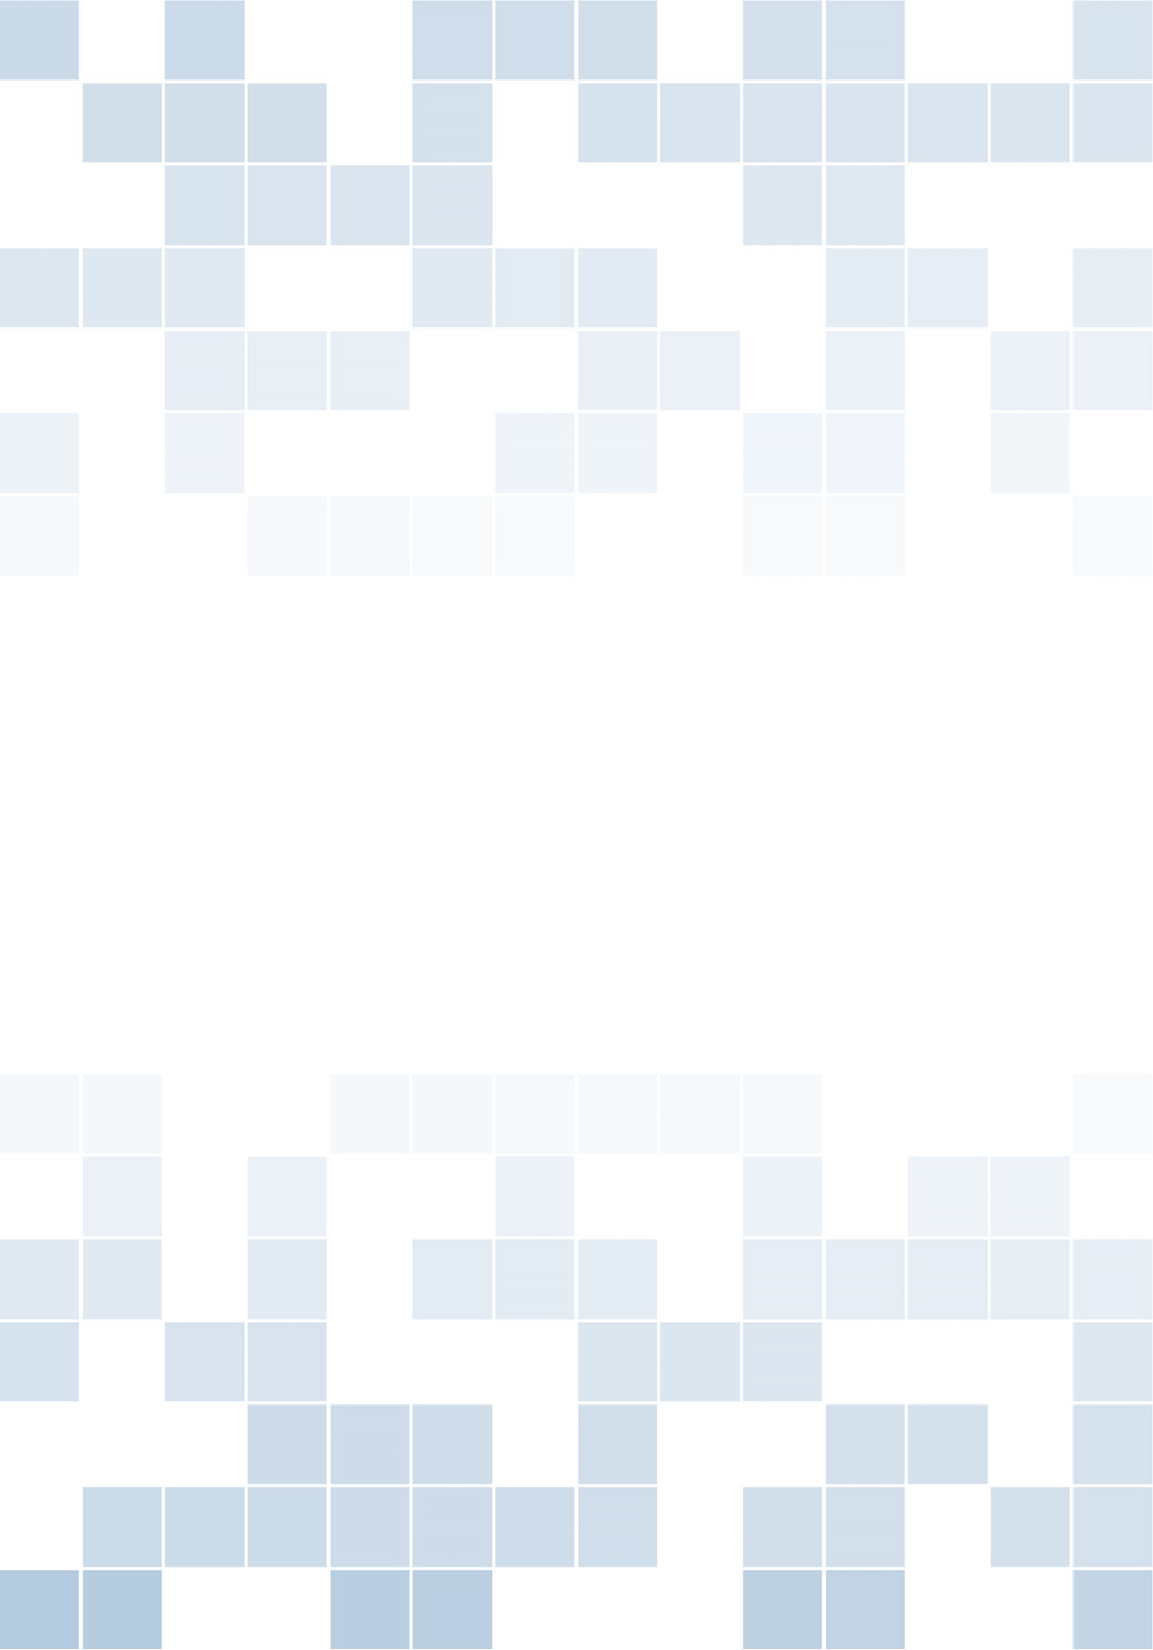
\includegraphics[width=\paperwidth]{background.pdf}};
\draw (current page.center) node [fill=ocre!30!white,fill opacity=0.6,text opacity=1,inner sep=1cm]{\Huge\centering\bfseries\sffamily\parbox[c][][t]{\paperwidth}{\centering Statistical Process Control in Healthcare\\[15pt] % Book title
{\large November 2019}\\[20pt] % Subtitle
{\Large Sydney Paul, Dwight Barry, Brendan Bettinger, and Andrew Cooper}}}; % Author name
\end{tikzpicture}
\end{titlepage}

{
\hypersetup{linkcolor=black}

%----------------------------------------------------------------------------------------
%	TABLE OF CONTENTS
%----------------------------------------------------------------------------------------

\setcounter{tocdepth}{2}

\chapterimage{chapter_head_1.pdf}

\pagestyle{empty} % Disable headers and footers for the following pages

\tableofcontents % Print the table of contents itself

\pagestyle{fancy} % Enable headers and footers again
}

\makeatletter
\let\stdchapter\chapter
\renewcommand*\chapter{%
  \@ifstar{\starchapter}{\@dblarg\nostarchapter}}
\newcommand*\starchapter[1]{\usechapterimagefalse\stdchapter*{#1}\usechapterimagetrue}
\def\nostarchapter[#1]#2{\chapterimage{chapter_head_2.pdf}\stdchapter[{#1}]{#2}}
\makeatother


\hypertarget{output}{%
\chapter{output:}\label{output}}

Placeholder

\hypertarget{preface_problem}{%
\section{We have a problem}\label{preface_problem}}

\hypertarget{preface_questions}{%
\section{Common questions}\label{preface_questions}}

\hypertarget{who-is-this-book-for}{%
\subsection*{\texorpdfstring{\emph{Who is this book for?}}{Who is this book for?}}\label{who-is-this-book-for}}
\addcontentsline{toc}{subsection}{\emph{Who is this book for?}}

\hypertarget{what-do-i-need-to-start}{%
\subsection*{\texorpdfstring{\emph{What do I need to start?}}{What do I need to start?}}\label{what-do-i-need-to-start}}
\addcontentsline{toc}{subsection}{\emph{What do I need to start?}}

\hypertarget{preface_about}{%
\section{About}\label{preface_about}}

\hypertarget{who-are-we}{%
\subsection*{\texorpdfstring{\emph{Who are we?}}{Who are we?}}\label{who-are-we}}
\addcontentsline{toc}{subsection}{\emph{Who are we?}}

\hypertarget{what-if-i-find-a-typo}{%
\subsection*{\texorpdfstring{\emph{What if I find a typo?}}{What if I find a typo?}}\label{what-if-i-find-a-typo}}
\addcontentsline{toc}{subsection}{\emph{What if I find a typo?}}

\hypertarget{step-1-load-your-file}{%
\chapter*{Step 1: Load your file}\label{step-1-load-your-file}}
\addcontentsline{toc}{chapter}{Step 1: Load your file}

Placeholder

\hypertarget{parameters}{%
\chapter{Step 2: Set your parameters}\label{parameters}}

Placeholder

\hypertarget{eda_assumptions}{%
\chapter{Step 2: Exploratory Data Analysis and Checking Assumptions}\label{eda_assumptions}}

Placeholder

\hypertarget{exploratory-data-analysis}{%
\section{Exploratory Data Analysis}\label{exploratory-data-analysis}}

\hypertarget{checking-assumptions}{%
\section{Checking Assumptions}\label{checking-assumptions}}

\hypertarget{run_chart}{%
\chapter{Run Chart}\label{run_chart}}

Placeholder

\hypertarget{control_chart}{%
\chapter{Control Chart}\label{control_chart}}

The primary distinction between run and control charts is that the latter uses parametric statistics monitor additional properties of a data-defined process. If a particular statistical distribution---such as normal, binomial, or Poisson---matches the process you wish to measure, a control chart offers a great deal more power to find insights and monitor change than a line or run chart. Parametric distributions are a \emph{useful fiction}---no data will follow an idealized distribution, but as long as it's close, the distribution properties provide useful shortcuts that allow SPC charts to work \emph{in practice}.

There are \href{https://en.wikipedia.org/wiki/List_of_probability_distributions}{hundreds of statistical distributions}, but only a handful are commonly used in SPC work:

\begin{longtable}[]{@{}llllll@{}}
\toprule
\begin{minipage}[b]{0.16\columnwidth}\raggedright
Data Type\strut
\end{minipage} & \begin{minipage}[b]{0.22\columnwidth}\raggedright
Distribution\strut
\end{minipage} & \begin{minipage}[b]{0.09\columnwidth}\raggedright
Range\strut
\end{minipage} & \begin{minipage}[b]{0.07\columnwidth}\raggedright
Skew\strut
\end{minipage} & \begin{minipage}[b]{0.13\columnwidth}\raggedright
Example\strut
\end{minipage} & \begin{minipage}[b]{0.16\columnwidth}\raggedright
SPC chart\strut
\end{minipage}\tabularnewline
\midrule
\endhead
\begin{minipage}[t]{0.16\columnwidth}\raggedright
\emph{Discrete}\strut
\end{minipage} & \begin{minipage}[t]{0.22\columnwidth}\raggedright
Binomial\strut
\end{minipage} & \begin{minipage}[t]{0.09\columnwidth}\raggedright
0, \(N\)\strut
\end{minipage} & \begin{minipage}[t]{0.07\columnwidth}\raggedright
Any\strut
\end{minipage} & \begin{minipage}[t]{0.13\columnwidth}\raggedright
Bundle compliance percentage\strut
\end{minipage} & \begin{minipage}[t]{0.16\columnwidth}\raggedright
\emph{p}, \emph{np}\strut
\end{minipage}\tabularnewline
\begin{minipage}[t]{0.16\columnwidth}\raggedright
\strut
\end{minipage} & \begin{minipage}[t]{0.22\columnwidth}\raggedright
Poisson\strut
\end{minipage} & \begin{minipage}[t]{0.09\columnwidth}\raggedright
0, \(\infty\)\strut
\end{minipage} & \begin{minipage}[t]{0.07\columnwidth}\raggedright
Right\strut
\end{minipage} & \begin{minipage}[t]{0.13\columnwidth}\raggedright
Infections per 1,000 line days\strut
\end{minipage} & \begin{minipage}[t]{0.16\columnwidth}\raggedright
\emph{u}, \emph{c}\strut
\end{minipage}\tabularnewline
\begin{minipage}[t]{0.16\columnwidth}\raggedright
\strut
\end{minipage} & \begin{minipage}[t]{0.22\columnwidth}\raggedright
Geometric\strut
\end{minipage} & \begin{minipage}[t]{0.09\columnwidth}\raggedright
0, \(\infty\)\strut
\end{minipage} & \begin{minipage}[t]{0.07\columnwidth}\raggedright
Right\strut
\end{minipage} & \begin{minipage}[t]{0.13\columnwidth}\raggedright
Number of surgeries between complications\strut
\end{minipage} & \begin{minipage}[t]{0.16\columnwidth}\raggedright
\emph{g}\strut
\end{minipage}\tabularnewline
\begin{minipage}[t]{0.16\columnwidth}\raggedright
\emph{Continuous}\strut
\end{minipage} & \begin{minipage}[t]{0.22\columnwidth}\raggedright
Normal\strut
\end{minipage} & \begin{minipage}[t]{0.09\columnwidth}\raggedright
\(-\infty\), \(\infty\)\strut
\end{minipage} & \begin{minipage}[t]{0.07\columnwidth}\raggedright
None\strut
\end{minipage} & \begin{minipage}[t]{0.13\columnwidth}\raggedright
Patient wait times\strut
\end{minipage} & \begin{minipage}[t]{0.16\columnwidth}\raggedright
\emph{I}, \(\bar{x}\), EWMA, CUSUM\strut
\end{minipage}\tabularnewline
\begin{minipage}[t]{0.16\columnwidth}\raggedright
\strut
\end{minipage} & \begin{minipage}[t]{0.22\columnwidth}\raggedright
Weibull\strut
\end{minipage} & \begin{minipage}[t]{0.09\columnwidth}\raggedright
0, \(\infty\)\strut
\end{minipage} & \begin{minipage}[t]{0.07\columnwidth}\raggedright
Right\strut
\end{minipage} & \begin{minipage}[t]{0.13\columnwidth}\raggedright
Time between antibiotic doses\strut
\end{minipage} & \begin{minipage}[t]{0.16\columnwidth}\raggedright
\emph{t}\strut
\end{minipage}\tabularnewline
\bottomrule
\end{longtable}

When control charts use the mean to create the center line, they use the arithmetic mean. Rather than using the \(\bar{x}\) abbreviation, these mean values are usually named for the type of chart (\emph{u}, \emph{p}, etc.) to emphasize the use of control limits that are \emph{not} based on the normal distribution. The variance used to calculate the control limits differs by distribution.

The first decision that you must make is the correct control chart for your data. The first thing on this section of the application is a handy flow chart to help you make that decision.

\begin{figure}

{\centering 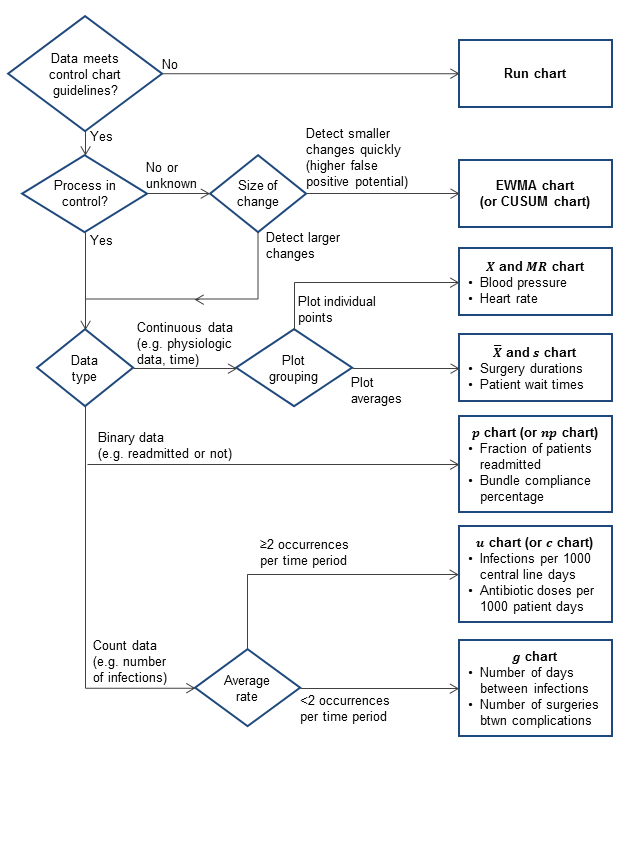
\includegraphics{control_chart_flowchart} 

}

\caption{Which control chart should I use?}\label{fig:unnamed-chunk-2}
\end{figure}

We will walk through the flow chart to answer this question for our example CLABSI data.

\emph{Does the data meet control chart guidelines?} Yes.
\emph{Size of change} We want to detect larger changes.
\emph{Data type} The data is count data.
\emph{Average rate} We have more than 2 occurrences per time period.

We want to use a \emph{u} chart! The flowchart also lists common applications for each type of chart. Our decision is backed up by the chart because `Infections per 1000 central line days' is a common reason for using a \emph{u} control chart.

Next we can scroll down to see a left-side panel with user options and inputs, the right-side panel is initially blank. The first option to select on the left panel is ``Choose your control chart''. Find the chart that you chose using the flowchart and select it. This will create your control chart on the right-side panel. We have chosen to use a u-chart for our example CLABSI data which can be seen in the figure below. Once again, each department has its own control chart for comparison.

\begin{figure}

{\centering 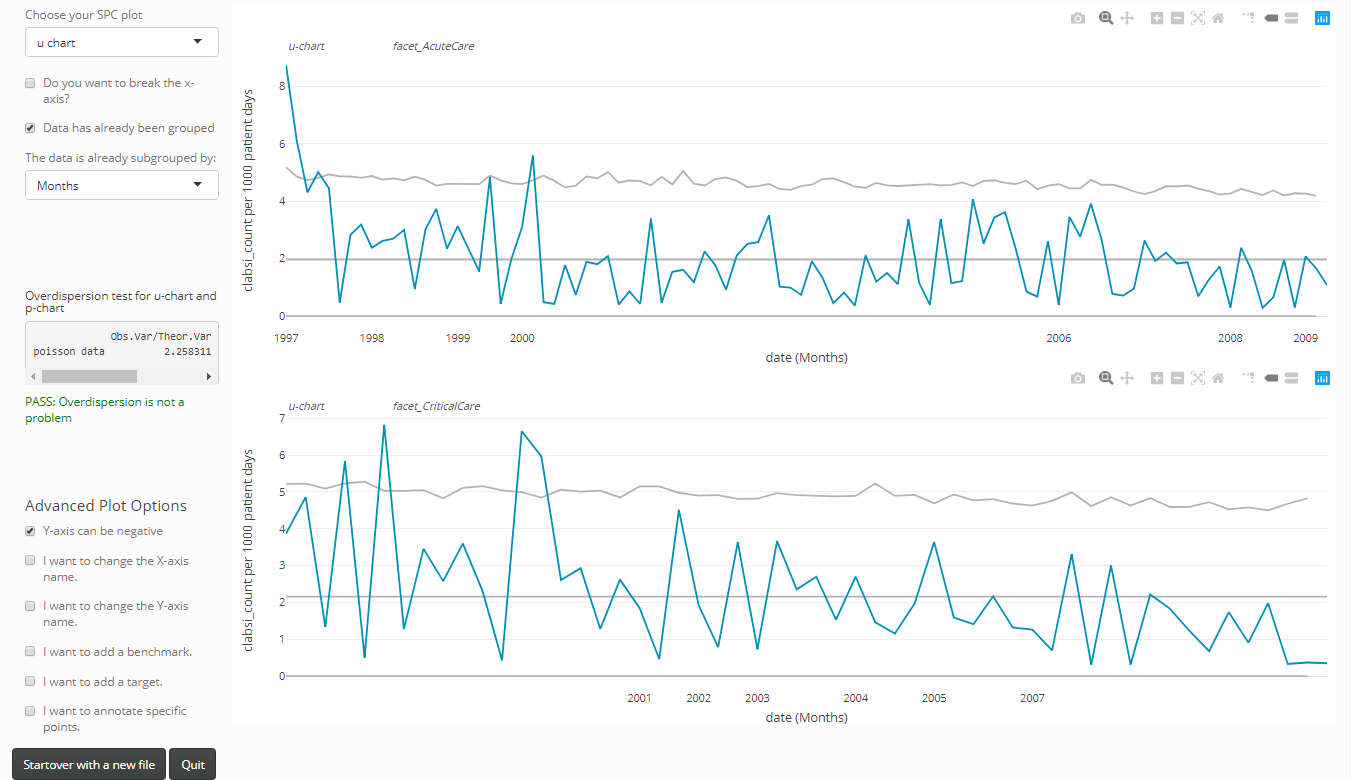
\includegraphics{step5_control_chart} 

}

\caption{u-charts for CLABSI data by department}\label{fig:unnamed-chunk-3}
\end{figure}

The next option on the left-side panel is a checkbox that asks ``Do you want to break the x-axis?''. To break the axis means to set a point in which different control limits are calculated before and after. This can be a column in your data containing time groupings, like ``pre-implementation'' and ``post-implementation'' \emph{or} you can select ``Choose date on calendar''. In the figure below, we have checked the box to break the x-axis. Then we selected Choose date on calendar". Using the calendar that pops up, we selected June 17th, 2004. If you look at this date on the control charts, you can see where the axis was broken. The change in control limits at that date is more noticeably for Critical Care than for Acute Care.

\begin{figure}

{\centering 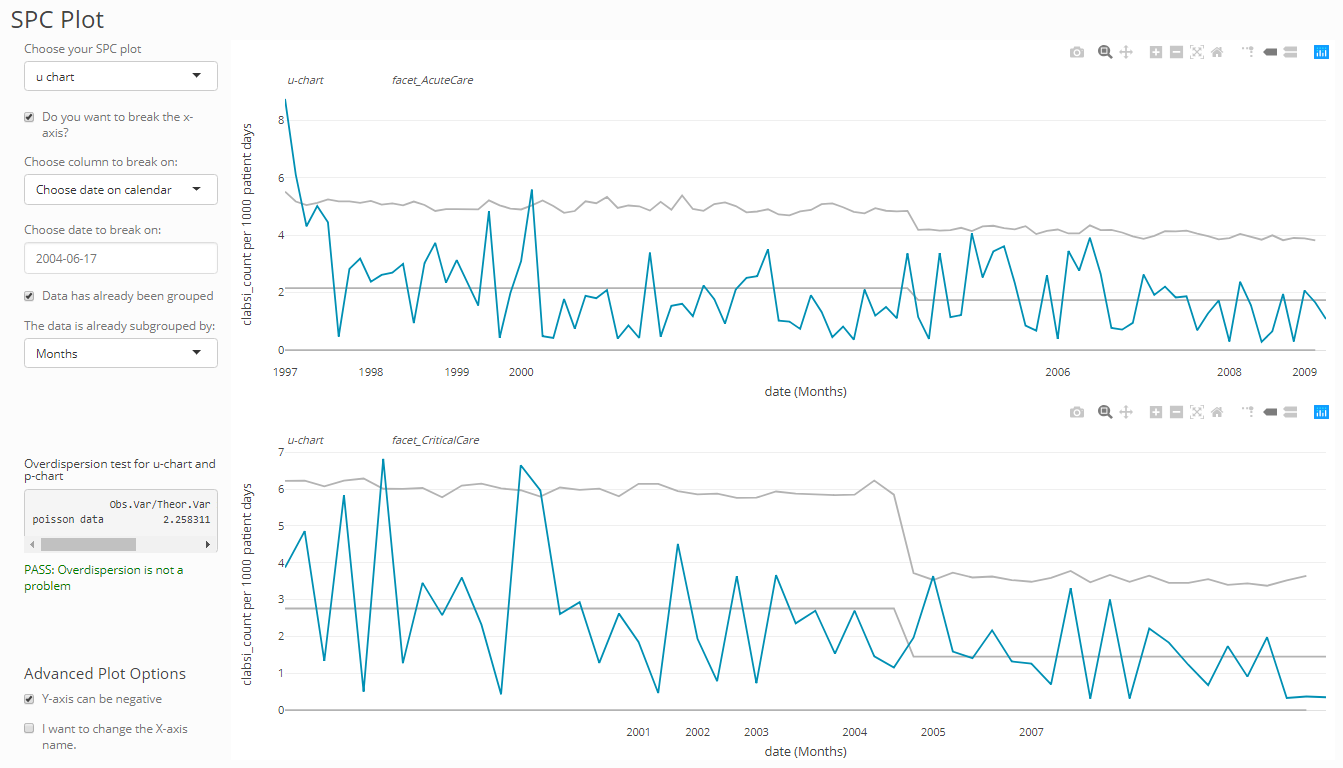
\includegraphics{step5_break_axis} 

}

\caption{u-charts for CLABSI data by department}\label{fig:unnamed-chunk-4}
\end{figure}

The next option is a checkbox labelled ``Data has already been grouped''. Below this is a drop down box containing various time aggregates. If the data has already been group, then you can use the drop down to select how it is being group. If you wish to change the aggregation of the data, then you can \emph{uncheck} this box. This changes the drop-down box to ``The data needs to be subgrouped by:'' where you can select your desired aggregation. The example CLABSI data was already aggregated by month, so we cannot go backwards into weeks or days. However, we can view the data aggregated by quarters instead.

\begin{figure}

{\centering 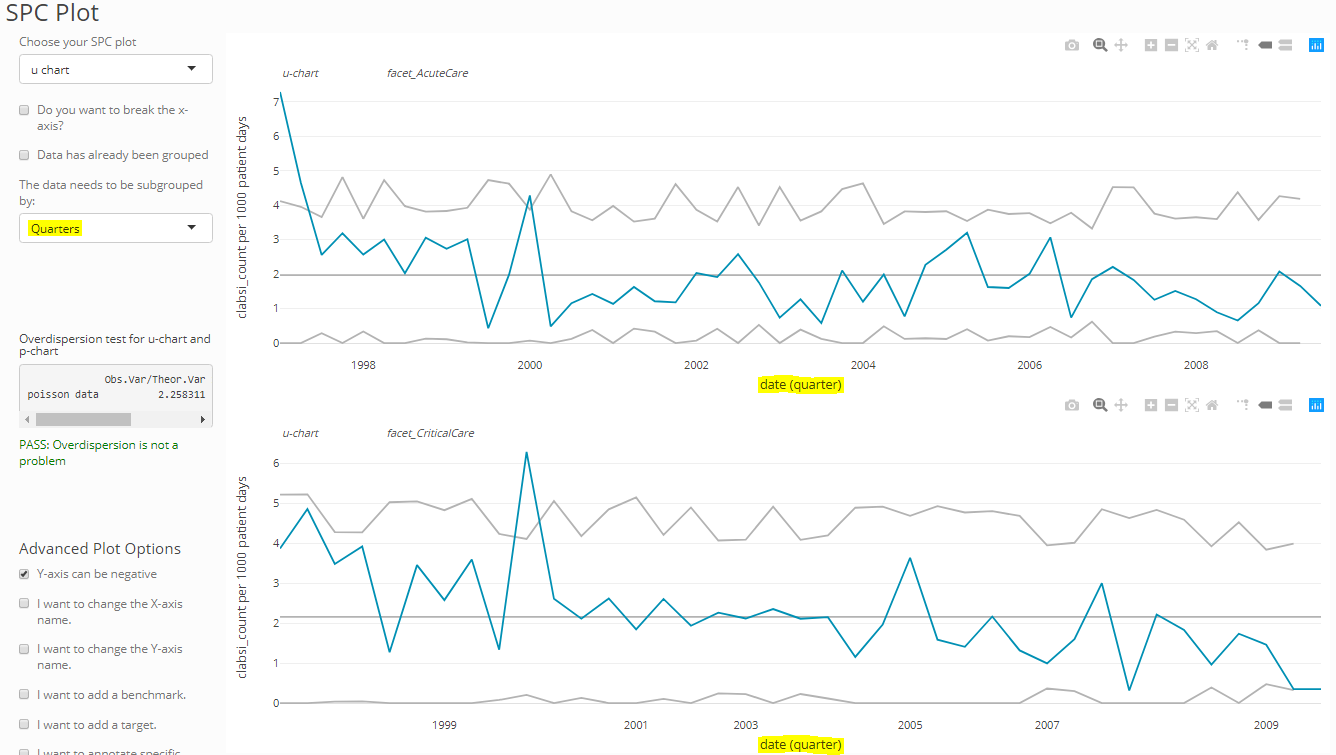
\includegraphics{step5_agg_quarter} 

}

\caption{u-charts for CLABSI data aggregated by quarter}\label{fig:unnamed-chunk-5}
\end{figure}

Be careful that you do not render your data useless by aggregation. When you aggregate, you lose information, and if you do not have enough observations you may miss what your data is trying to say. An example of too much aggregation is our same example CLABSI data aggregated by year.

\begin{figure}

{\centering 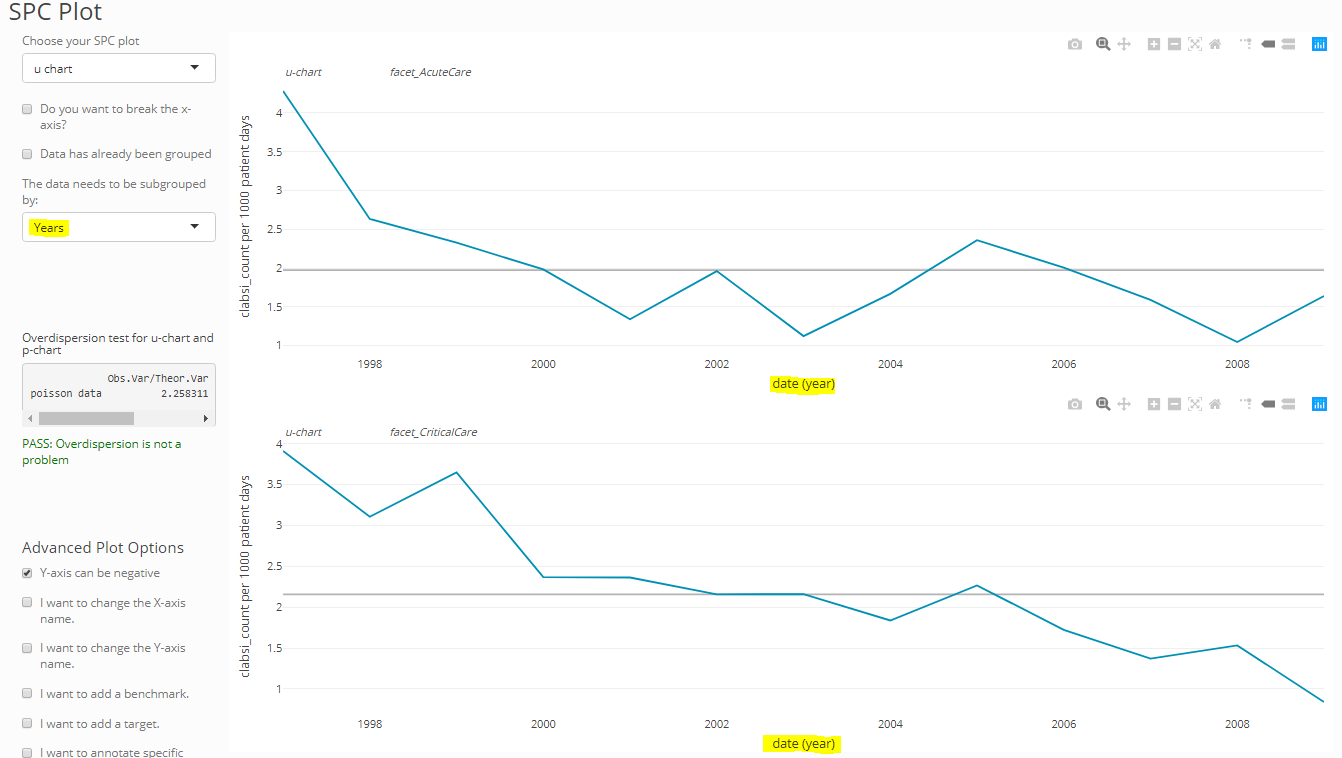
\includegraphics{step5_agg_year} 

}

\caption{u-charts for CLABSI data aggregated by year}\label{fig:unnamed-chunk-6}
\end{figure}

Moving down the left-side panel, the next thing we see is the ``Overdispersion test for u-chart and p-chart''. This only applies to these two charts. If overdispersion is a problem, which will be indicated in red text, then you should use prime charts instead, i.e.~a u' chart instead of u chart and p' chart instead of p chart. These are both available in the ``Choose your control chart'' drop-down box.

The final set of options are called ``Advanced Plot Options'' and are completely optional. Here you can prevent the y-axis from being negative (depending on your use-case) by unchecking the box. You can enter your own custom labels for the axes by checking the corresponding boxes and simply typing your desired lables. If you have a benmark value or target value, you can check those corresponding boxes and simply enter the desired numbers. Finally, if you wish to annotate you plot you can check the box labelled ``I want to annotate specific points''. This feature is only available for single plots (not comparing across groups like we did in the CLABSI example). A table of all your data will appear below your control chart. Simply double-click into the ``annotations'' column at the row you wish to annotate. Type in your annotation. When finished, use Ctrl and Enter simultaneously to finish editing the text box. Your annotation will appear as a number, with the text appearing when hovered over.

An example of these features in use can be seen below.

\begin{figure}

{\centering 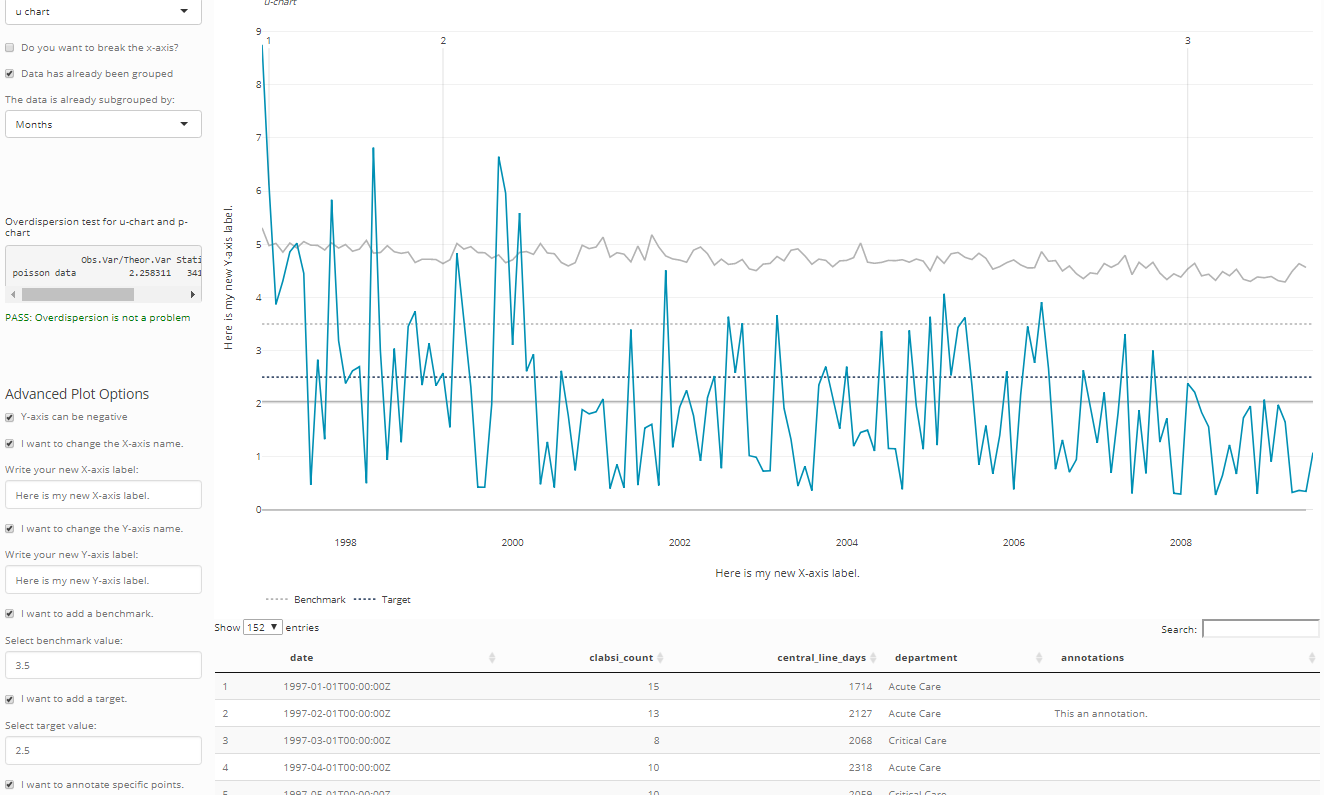
\includegraphics{step5_advanced_plot_options} 

}

\caption{u-chart for full dataset with advanced plot options}\label{fig:unnamed-chunk-7}
\end{figure}

Custom axes labels have been specified. A benchmark value has been set at 3.5, and a target value set at 2.5. These appear on the graph as dashed lines (grey and navy respectively) and have their own legend. Finally three annotations have been added using the table below. On the graph these appear as ``1'', ``2'', and ``3'' with vertical lines to the point they belong to. When you hover over each annotation number, you can see the full text.

At the very bottom are two options. You can either choose to start the application over with a new file, or you may quit and close the application. This ends the tutorial on using the accompanying SPC Shiny App. Over the next few chapters we will delve deeper into control charts and how to interpret them.

\hypertarget{part-part-i}{%
\part{Part I}\label{part-part-i}}

\hypertarget{ch1_commonMistakes}{%
\chapter{Common Mistakes in SPC}\label{ch1_commonMistakes}}

Placeholder

\hypertarget{mistake-1}{%
\section{Mistake \#1}\label{mistake-1}}

\hypertarget{ch1_mistake1}{%
\subsection*{Not using all the information that you have available to you}\label{ch1_mistake1}}
\addcontentsline{toc}{subsection}{Not using all the information that you have available to you}

\hypertarget{mistake-2}{%
\section{Mistake \#2}\label{mistake-2}}

\hypertarget{ch1_mistake2}{%
\subsection*{\texorpdfstring{Forgetting that SPC charts cannot make decisions for you, they can only help \emph{you} to make a decision}{Forgetting that SPC charts cannot make decisions for you, they can only help you to make a decision}}\label{ch1_mistake2}}
\addcontentsline{toc}{subsection}{Forgetting that SPC charts cannot make decisions for you, they can only help \emph{you} to make a decision}

\hypertarget{mistake-3}{%
\section{Mistake \#3}\label{mistake-3}}

\hypertarget{ch1_mistake3}{%
\subsection*{Skipping to the end of the process}\label{ch1_mistake3}}
\addcontentsline{toc}{subsection}{Skipping to the end of the process}

\hypertarget{mistake-4}{%
\section{Mistake \#4}\label{mistake-4}}

\hypertarget{ch1_mistake4}{%
\subsection*{Not understanding what it means to have a ``stable'' process}\label{ch1_mistake4}}
\addcontentsline{toc}{subsection}{Not understanding what it means to have a ``stable'' process}

\hypertarget{part-part-iii}{%
\part{Part III}\label{part-part-iii}}

\hypertarget{common_confusion}{%
\chapter{Run Charts vs.~Control Charts}\label{common_confusion}}

Placeholder

\hypertarget{run_or_control_chart}{%
\section{Which should I use: a run chart or a control chart?}\label{run_or_control_chart}}

\hypertarget{guidelines}{%
\section{Guidelines for interpreting SPC charts}\label{guidelines}}

\hypertarget{guide_controlCharts}{%
\chapter{A Guide to Control Charts}\label{guide_controlCharts}}

Placeholder

\hypertarget{types_controlCharts}{%
\section{Types of Control Charts}\label{types_controlCharts}}

\hypertarget{u-chart-example}{%
\subsection{\texorpdfstring{\emph{u}-chart example}{u-chart example}}\label{u-chart-example}}

\hypertarget{p-chart-example}{%
\subsection{\texorpdfstring{\emph{p}-chart example}{p-chart example}}\label{p-chart-example}}

\hypertarget{g-chart-example}{%
\subsection{\texorpdfstring{\emph{g}-chart example}{g-chart example}}\label{g-chart-example}}

\hypertarget{c--and-np-chart-details}{%
\subsection{\texorpdfstring{\emph{c}- and \emph{np}-chart details}{c- and np-chart details}}\label{c--and-np-chart-details}}

\hypertarget{i-mr-chart}{%
\subsection{\texorpdfstring{\emph{I-MR} chart}{I-MR chart}}\label{i-mr-chart}}

\hypertarget{barx-and-s-chart}{%
\subsection{\texorpdfstring{\(\bar{x}\) and \emph{s} chart}{\textbackslash{}bar\{x\} and s chart}}\label{barx-and-s-chart}}

\hypertarget{t-chart-example}{%
\subsection{\texorpdfstring{\emph{t}-chart example}{t-chart example}}\label{t-chart-example}}

\hypertarget{tips_tricks_controlCharts}{%
\section{Tips and tricks for successful control chart use}\label{tips_tricks_controlCharts}}

\hypertarget{when-to-revise-control-limits}{%
\subsection{When to revise control limits}\label{when-to-revise-control-limits}}

\hypertarget{custom_SPC_function}{%
\section{Custom SPC function}\label{custom_SPC_function}}

\hypertarget{ewma-chart}{%
\subsection{EWMA chart}\label{ewma-chart}}

\hypertarget{cusum-chart}{%
\subsection{CUSUM chart}\label{cusum-chart}}

\hypertarget{additional_resources}{%
\chapter{Additional Resources}\label{additional_resources}}

Placeholder

\hypertarget{time_series}{%
\section{Time series EDA}\label{time_series}}

\hypertarget{trend}{%
\subsection{Trend}\label{trend}}

\hypertarget{seasonplot}{%
\subsection{Seasonplot}\label{seasonplot}}

\hypertarget{monthplot}{%
\subsection{Monthplot}\label{monthplot}}

\hypertarget{autocorrelation}{%
\subsection{Autocorrelation}\label{autocorrelation}}

\hypertarget{cycles}{%
\subsection{Cycles}\label{cycles}}

\hypertarget{decomposition}{%
\subsection{Decomposition}\label{decomposition}}

\hypertarget{seasonal-adjustment}{%
\subsection{Seasonal adjustment}\label{seasonal-adjustment}}

\hypertarget{residuals}{%
\subsection{Residuals}\label{residuals}}

\hypertarget{accumuluation-plots}{%
\subsection{Accumuluation plots}\label{accumuluation-plots}}

\hypertarget{code_customSPC_function}{%
\section{Custom SPC Function}\label{code_customSPC_function}}

\hypertarget{code_examples}{%
\section{Code used to generate examples}\label{code_examples}}

\hypertarget{useful_resources}{%
\section{Useful References}\label{useful_resources}}

\hypertarget{useful_resources}{%
\section{Useful References}\label{useful_resources}}


\end{document}
